\section{BioMérieux Biopedia}
\label{biomerieuxBiopedia}

\begin{figure}[h]
    \centering
    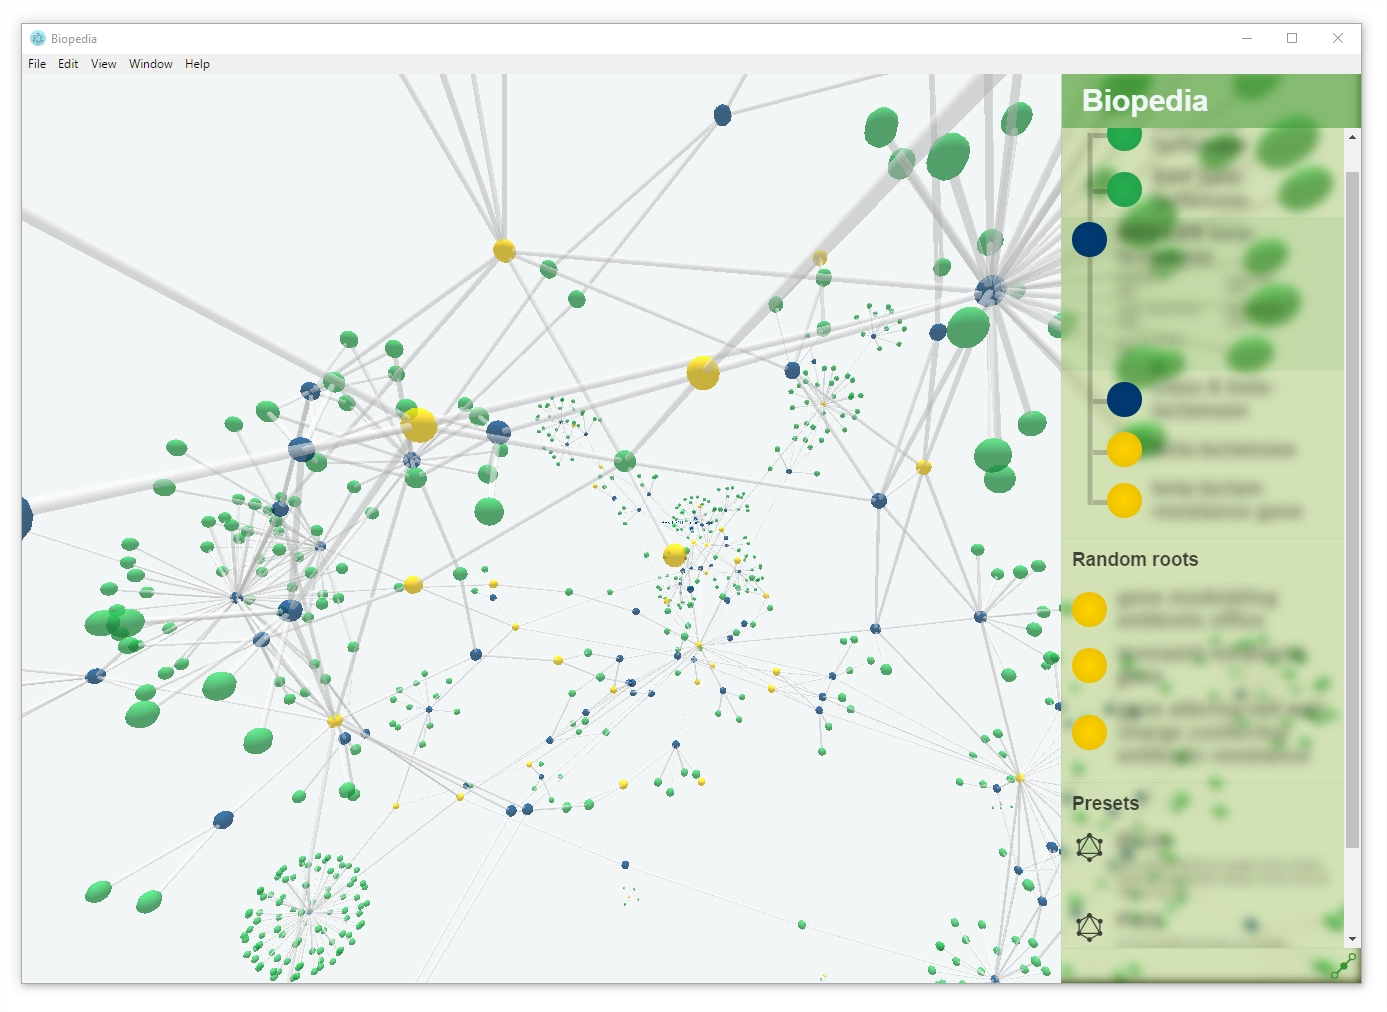
\includegraphics[scale=0.35]{img/Biopedia.jpg}
    \caption{Capture d'écran de la version actuelle de Biopedia}
\end{figure}

L'objectif de cette application est de présenter les données d'une base de données de BioMérieux sous forme de graphe pour la présentation aux clients intéressés.

Au moment où j'écris ces lignes, je suis toujours en train de développer activement cette application pour la présenter au client final le 20 avril;
Certaines informations pourront alors changer à l'avenir.

\subsection{Application précédente}
\label{biomerieuxBiopediaApplicationPrécédente}

Cela longtemps que LTBL à ce projet de visualisation de graphes et une première version a déjà été présentée.
Mais cette application se basait sur une vieille librairie et de nouvelles fonctionnalités ont été demandées par le client.

Apres, une étude du code de cette application nous avons décidé de le revoir complètement.
Je me suis donc lancé sur la création d'une toute nouvelle application de visualisation.

Cette application devra disposer des fonctionnalités suivantes :

\begin{itemize}
    \item Afficher les données dans un graphe en 3 dimensions
    \item Afficher les noms des noeuds du graphe quand on clique dessus
    \item Afficher les parents et enfants de ce noeud lors de la sélection
    \item Naviguer aisément dans les données
    \item Afficher une portion du graphe uniquement dans le cadre d'une étude de cas
\end{itemize}

\subsection{Technologies}
\label{biomerieuxBiopediaTéchnologies}

Pour créer cette application, je me suis tout d'abord tourné vers Unity\footnote{Unity est un moteur de jeu permettant d'afficher dans une scène en 3D des structures associées à des matériaux.} Pour la création d'un environnement en trois dimensions.
Unity permet d'avoir des environnements 3D très interactifs et faciles à utiliser.
Mais j'ai aussi remarqué un manque évident de librairies permettant de créer des graphes comme dans l'ancienne version de Biopedia.
De plus, je n'allais pas passer les trois semaines dédiés à ce projet pour la recréation d'un graphique de ce type.

J'ai donc décidé de retourner sur une solution Web avec Electron et les WebComponents.
Pour ce faire, j'ai utilisé la librairie \emph{3d-force-graph} se basant sur \emph{ThreeJS} pour l'affichage en 3D dans un Canvas WebGL .

\emph{ThreeJs} est la principale librairie permettant de concevoir des scènes en 3D avec WebGL .
Elle permet de placer des primitives dans la scène 3D et de faire diverses actions comme des mouvements de caméra, l'utilisation de matériaux et la création d'animations.
Dans mon cas, je l'utilise pour représenter le graphique des données.

\subsection{Force-directed graph}
\label{biomerieuxBiopediaForceDirectedGraph}

Les données de BioMérieux sont des données réparties en Graph.
Cela signifie que ce sont des données représentées par un ensemble de \emph{noeuds} reliés ensemble par des \emph{Relations}.
Les relations de ce graphe sont orientées, c'est-à-dire qu'elles disposent d'un noeud source et d'un noeud cible.
Ce type de graphe peut être représenté de multiples manières, mais la technique que j'ai utilisée ici est la technique du \emph{Force-directed Graph}.

Cette technique consiste à considérer chaque noeud comme un objet physique dans l'espace (ou le plan suivant le nombre de dimensions) et chaque relation comme un ressort reliant les noeuds.
On applique alors des forces sur les noeuds et on applique les lois de la physique au fil du temps pour obtenir un rendu graphiquement plaisant.
Cela peut prendre un certain temps avant d'avoir un résultat satisfaisant, car ce système est itératif.
Il nécessite alors une évolution du graphe jusqu'à atteindre un état de stabilité.

Je me suis intéressé à la simulation de ce genre de système pour l'implémenter dans Unity, mais due à un deadline assez proche, j'ai été obligé de trouver une librairie proposant une simulation de la position des noeuds.

\subsubsection{Nomenclature}
\label{biomerieuxBiopediaNomenclature}

Le graphe de BioMérieux dispose d'une nomenclature spécifique permettant de repérer les différents éléments.
Dans notre cas, les couleurs montrent la position des noeuds dans l'arborescence et non un type particulier.

\begin{description}
    \item[Noeud vert] Représente une feuille du graphe soit un noeud qui ne dispose que de relations dans sa direction et aucune relation ne partant de ce noeud
    \item[Noeud bleu] Représente un noeud intermédiaire soit un noeud disposant de relations depuis et vers lui
    \item[Noeud jaune] Représente un noeud racine soit un noeud qui ne dispose d'aucune relation dans sa direction
\end{description}

Chaque noeud de Biopedia dispose de métadonnées donnant plus d'informations sur le noeud actuellement sélectionné.

\subsection{Structure}
\label{biomerieuxBiopediaStructure}

\begin{figure}[h]
    \centering
    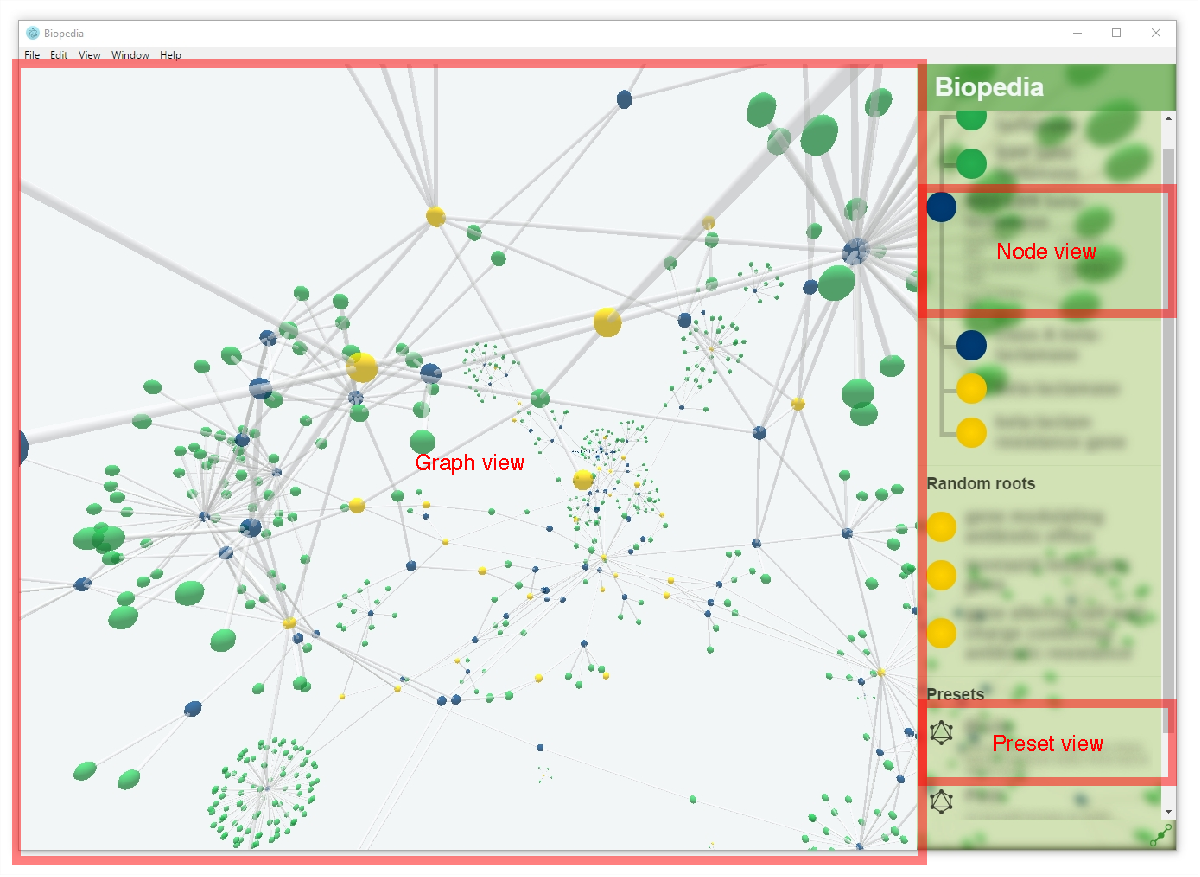
\includegraphics[scale=0.8]{img/biopedia-structure.pdf}
    \caption{Structure de l'application Biopedia}
\end{figure}

Dans cette application, j'utilise toutes les compétences acquises durant les projets précédents pour concevoir cette application de manière flexible pour qu'il soit aisé de comprendre mon code et d'ajouter des fonctionnalités à l'avenir.

\clearpage

Les différents \components composant cette application sont les suivants :

\paragraph{Graph view} Le lecteur de graphique permettant d'afficher un graphique des données en 3 dimensions a l'aide de \emph{ThreeJs}.
Il est possible de cliquer sur les noeuds du graphique pour le sélectionner et afficher diverses informations dans la barre de contrôle présente sur la droite de l'interface.

\paragraph{Node view} En charge de formater l'affichage d'un noeud sur l'interface.
Ce component est totalement indépendant des autres et permet juste d'afficher un noeud avec un design constant.
Il est utilisé pour afficher le noeud sélectionné avec les diverses métadonnées qui lui sont associées dans la barre de contrôle.
Mais il est aussi utilisé dans la liste de noeuds aléatoire permettant de rapidement démarrer une navigation dans le graphique.

\paragraph{Preset view} Dans le même objectif d'unifier le design de l'affichage des différents presets, ce component sert à afficher un preset à l'utilisateur.
Il est utilisé dans la barre de contrôle et permet de sélectionner un preset pour filtrer l'affichage des données dans le graphe.

\subsection{Conclusion}
\label{biomerieuxBiopediaConclusion}

Ce projet n'étant pas encore fini, certaines informations et structures peuvent changer.
Mais ce projet m'a permis de revoir mon évolution et les compétences acquises durant mon stage.
De plus, j'ai eu l'occasion de découvrir la 3D dans le navigateur avec ThreeJs et les simulations de graphiques en 3 dimensions.
Ce projet fut très instructif et unique comme tous les projets chez LTBL.
